\documentclass[ignorenonframetext,notes, 10pt, aspectratio=169]{beamer}

\usepackage{preamble_slides}


\title{\textbf{\Large{Introduction to git for social science students}}}
\providecommand{\subtitle}[1]{}
\subtitle{(not software developers)}
\author{Shiro Kuriwaki}
\date{March 5, 2019}

\begin{document}

\begin{frame}{Setup}
\begin{columns}[T]
\begin{column}{0.6\textwidth}
\begin{wideenumerate}
\item Go to \url{www.github.com} and make a free account
% https://happygitwithr.com/github-acct.html#username-advice
\item Make sure you have a recent version (v1.1 or later) of RStudio \url{https://www.rstudio.com/products/rstudio/download/\#download}
\item Keep \url{www.happygitwithr.com} open
\end{wideenumerate}
\end{column}
\begin{column}{0.4\textwidth}
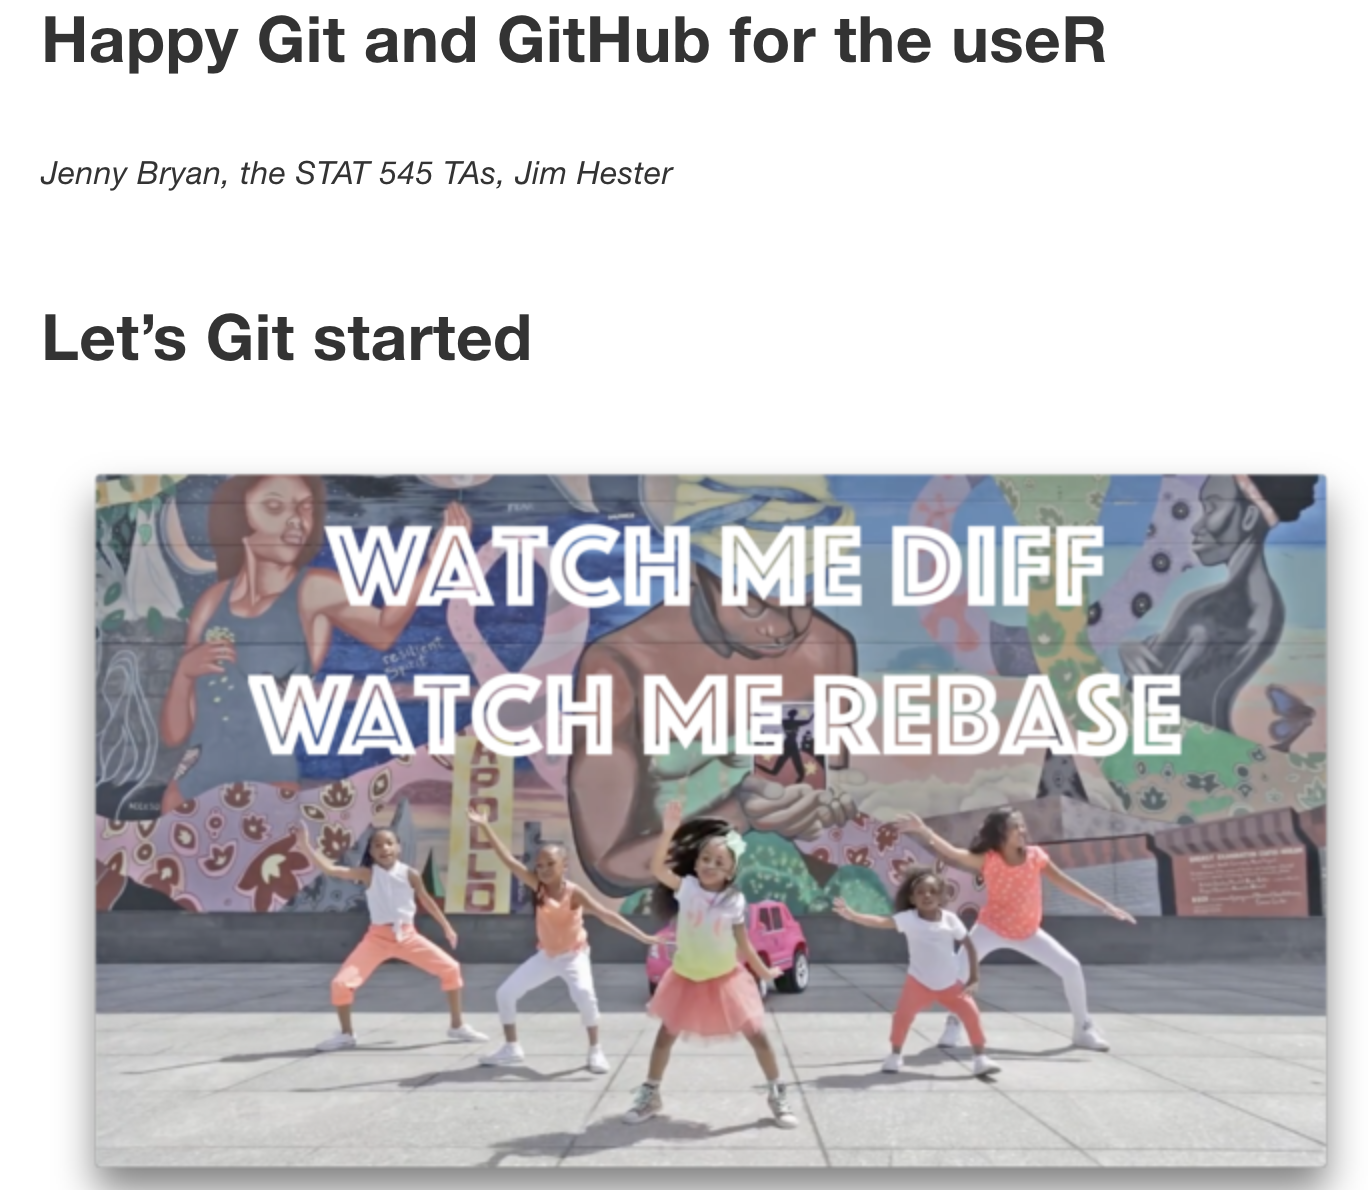
\includegraphics[width = \linewidth]{happygit.png}
\end{column}
\end{columns}
\end{frame}

\begin{frame}
\centering
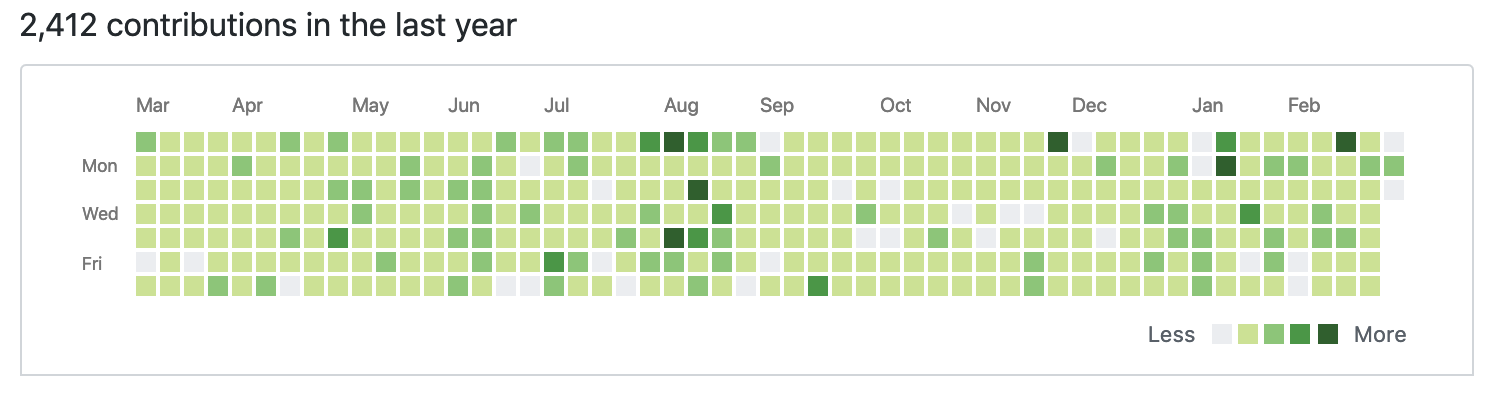
\includegraphics[width = 0.9\linewidth]{portfolio.png}
\maketitle
\end{frame}



\begin{frame}{Thanks for having me}

\begin{columns}[T]

\begin{column}{0.5\textwidth}
\bfheading{About me}
\begin{wideitemize}
\item G-4 in Government
\item American Politics, elections and representation
\item Before: A year in political data analytics (where I learned git from \href{https://anniejw.com/}{Annie Wang})
\end{wideitemize}\pause

\begin{wideitemize}
\item I do some software development, 
\item but most of my work is applied (``substantive'')
\end{wideitemize}
\end{column}\pause
\begin{column}{0.5\textwidth}
\bfheading{My perspective}
\begin{wideitemize}
\item Version control is mandatory for programmers\pause
\item but does it make sense for \emph{applied} researchers
\item who work with datasets that are \pause ~\alert{large},\pause ~\alert{unstructured},\pause ~\alert{prone to change},\pause ~\alert{with collaborators}
\end{wideitemize}
\end{column}
\end{columns}
\end{frame}

\begin{frame}{Setting Expectations: Is it worth it?}
\begin{columns}[T]
\begin{column}{0.5\textwidth}
\bfheading{What do Gentzkow and Shapiro say?}

Definitely:
\begin{quote}
``It will probably take you a couple days to set up a repository and learn how you want to interact with [Version Control]. You will break even on that time investment within a month or two.''\footnote[frame]{Code and Data for Social Sciences: A Practioners Guide. 2014. \url{https://perma.cc/5J9D-BTD6}.  \textcolor{gray}{Although I'm not sure about learning version control in ``a couple of days'' (I certainly couldn't!), I can guarantee reading their guide in its entirety \emph{is} a time investment you'll break even on immediately.}}
\end{quote}
\end{column}
\begin{column}{0.5\textwidth}
but also see\footnote[frame]{\url{https://community.rstudio.com/t/version-control-with-google-drive/4032}}
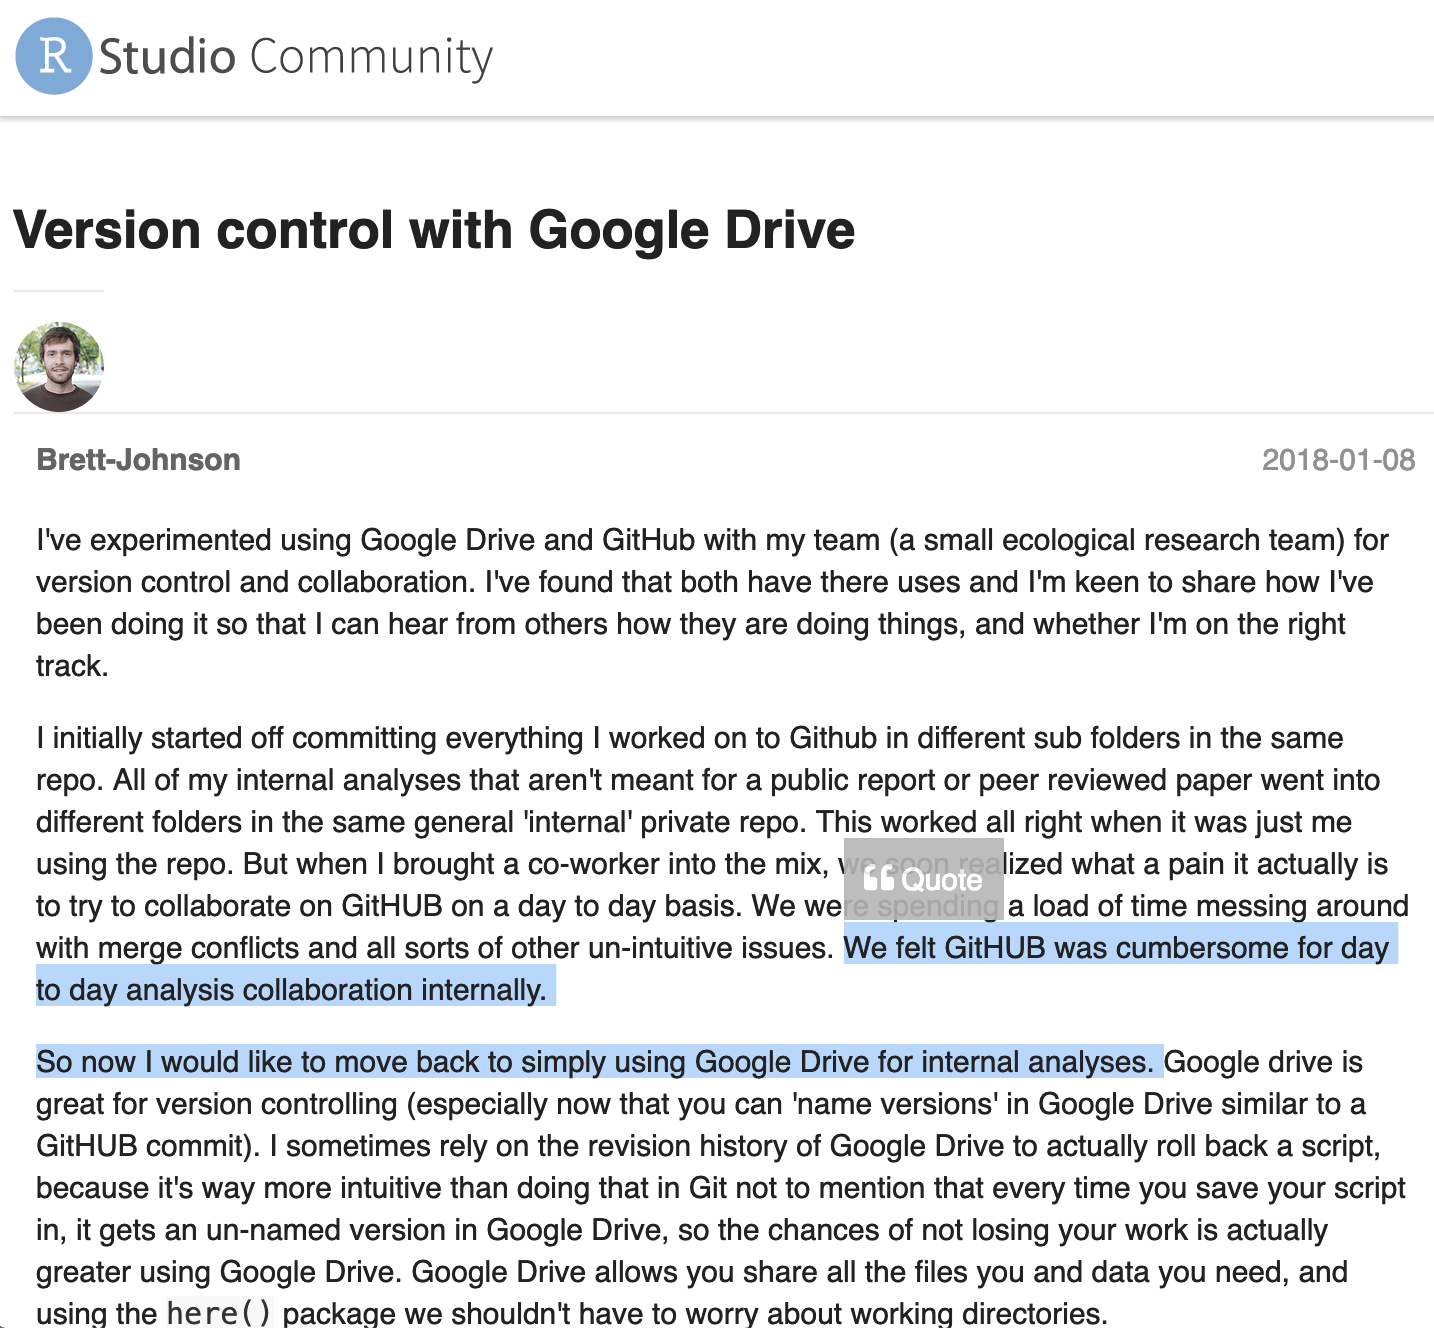
\includegraphics[width = 0.8\linewidth]{github_vs_gdrive.png}
\end{column}
\end{columns}
\end{frame}



\begin{frame}{My (recommended) setup}
\end{frame}


\begin{frame}{Terminology}
\begin{columns}[T]
\begin{column}{0.5\textwidth}
\begin{wideitemize}
\item \alert{Git} is a particular type of software for version control (Subversion is another)
\item \alert{GitHub} is an app (recently bought by Microsoft) to host git on the web (Bitbucket is another)
\item A \alert{desktop client} is an app that connects a webhost like Github to your computer and facilitates simple tasks (here I use \alert{RStudio}, there are many others)
\item A \alert{repository} is the fundamental unit of a version control, like a project folder. \pause Do not make a repository within a repository! 
\end{wideitemize}
\end{column}
\begin{column}{0.5\textwidth}
\end{column}
\end{columns}
\end{frame}



% \begin{frame}{Frame}
% \begin{columns}[T]
% \begin{column}{0.5\textwidth}
% \end{column}
% \begin{column}{0.5\textwidth}
% \end{column}
% \end{columns}
% \end{frame}


\begin{frame}{Summary and wider context}

\begin{tcolorbox}
Preference for local taxation and public goods provision is not partisan.  
\end{tcolorbox}
\pause
\small

\begin{columns}[T]
\begin{column}{0.2\textwidth}
\itheading{This project brings vote choice data into the debate of policy representation in a Federalist system:}

\end{column}
\begin{column}{0.4\textwidth}
\itheading{``The Increasingly United States''}

\begin{wideitemize}
\item State representatives \textcolor{gray}{(Rogers 2018)} and voters \textcolor{gray}{(Tausanovitch and Warshaw 2014)} oriented along national partisan lines
\item Accelerated by the nationalization of media \textcolor{gray}{(Hopkins 2018)}
\item But other dimensions do exist (in California?) \textcolor{gray}{(Snyder 1996, Gerber and Lewis  2004)}
\end{wideitemize}

\end{column}

\begin{column}{0.4\textwidth}
\itheading{``Something for Something''}

\begin{wideitemize}
\item Precincts vote for and against redistribution according to their needs \textcolor{gray}{(Sances 2018)}, and school elections hinge on school performance \textcolor{gray}{(Payson 2017, Kogan, Lavertu, Peskowitz 2015)}
\item Individual (voter-file) data reveals insights about who participates and how \textcolor{gray}{(Kogan, Lavertu, Peskowitz 2018)}
\end{wideitemize}
\end{column}
\end{columns}

\end{frame}

\end{document}
